\documentclass[runningheads,a4paper]{llncs}

\usepackage{graphicx}
\usepackage{wrapfig}
\usepackage{subfigure}
\usepackage[utf8]{inputenc}
\pagenumbering{roman}
\usepackage{textcomp}
\usepackage{pifont}
\usepackage{color}
\usepackage{blindtext}
\usepackage{enumitem}


\begin{document}
\mainmatter  % start of an individual contribution

%Titel
\title{HCI Meilenstein 1}

\titlerunning{HCI Meilenstein 2}

\author{
  Dursun, Camkerten
  \texttt{a0027244@@unet.univie.ac.at}
  \and
  Pektas, Tarik
  \texttt{a1325165@@unet.univie.ac.at}
  \and
  Bozkurt Yigit Berkay
  \texttt{a1029659@@unet.univie.ac.at}
  \and
  Ayyildiz Mert Ahmet
  \texttt{a1125172@@unet.univie.ac.at}
}

\institute{Universität Wien  / HCI \\
\ SS16 / Gruppe 3}


\maketitle

\section{Ideensammlung}
\subsection{Methodenwahl}
\subsection{Ergebnisse}

\clearpage

\section{Low-fi Prototypen}
\subsection{Prototyp-1}

Um die Effizienz zu steigern haben wir uns entschieden als Startseite die "Ausgaben Hinzufügen (Add Expense) " Funktion zu verwenden. Somit kann der User sofort die Hauptfunktion verwenden. 
Unser erster Prototyp listet die entsprechenden Felder welche für eine Ausgabe befüllt werden müssen auf. [a]
Links oben befindet sich ein Shortcut zum Side Panel. Nach einem Touch auf diesen "Bar" wird das seitliche Menü angezeigt [b]. Hier werden alle erreichbaren Menüpunkte aufgelistet. Dieser Side Panel ist von jeder Seite aus erreichbar.
Die "Income" Seite dient zur Speicherung eines neuen Einkommens. [c]\\Das Datum, die Menge und die Herkunft sollen hier durch Eingabe Felder abgefragt und gespeichert werden. Durch einen erneuten Aufruf des Side Panels kann man nun, unter anderem, die Report Seite aufrufen.[d]

\begin{figure}
\centering
\subfigure[Ausgabe hinzufügen]{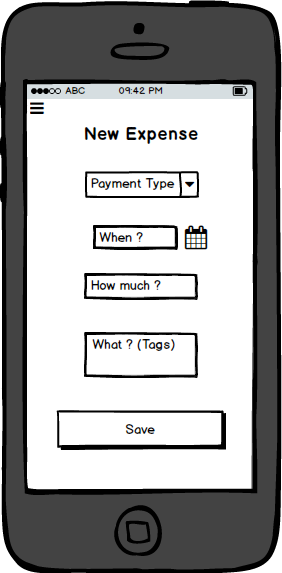
\includegraphics[width=0.20\textwidth]{Expense-1}}
\hfill
\subfigure[Side Panel]{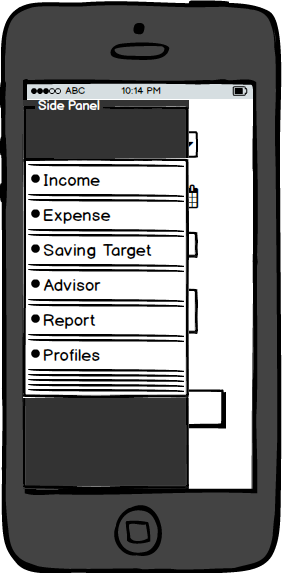
\includegraphics[width=0.20\textwidth]{SidePanel-1}}
\hfill
\subfigure[Enkommen Speichern]{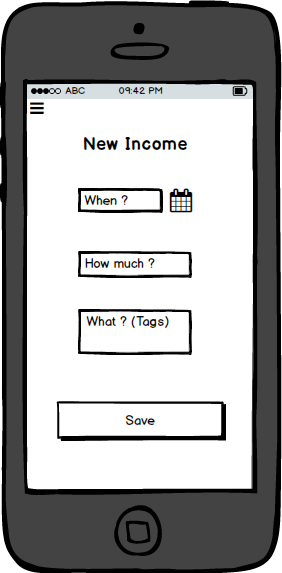
\includegraphics[width=0.20\textwidth]{Income-1}}
\hfill
\subfigure[Bericht erstellen]{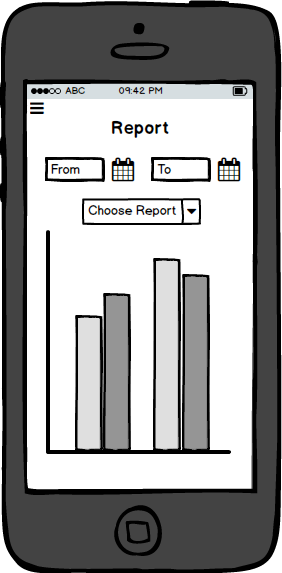
\includegraphics[width=0.20\textwidth]{Report-1}}
\end{figure}



Geplant ist das eine Datumseingabe mittels Start Datum und Enddatum sowie der Typ, durch eine Drop down Auswahl, selektiert werden um somit den entsprechenden Bericht auf der Seite wiederzugeben. Weiteres ist geplant eine Profil Seite zu erstellen [e]. 
Dieser soll durch einen Klick im Side Panel auf dem Menüpunkt "Profiles" erreicht werden.\\ Falls der User noch kein Profil hat kann er nun auf dieser Seite im Drop down Menü "Create New" auswählen welches automatisch auf die Seite "New Profile" weiterleiten wird [f].\\\\ Sollte der User bereits ein Profil haben kann er diesen durch die Auswahl [edit] neben dem Profilenamen im Dropdown die Seite zum Editieren erreichen[g]. Ein Alias für den aktuellen Account, der Name des Users sowie eine Standard Kreditkarten Nummer und die gewünscht Währung soll hier eingegeben werden. Ein weiterer wichtiger Menüpunkt und auch Usecase ist das Sparziel[h] \\Das Ziel dieser Funktion ist es den Nutzern zu ermöglichen Sparziele zu setzten. Diese werden durch die Eingabe des Ziels, das end Datum sowie die Materie selbst festgelegt. Wir planen diese Ziele im Report sowie im Advisor zur berücksichtigen. \\ Obwohl der Advisor nicht zu den primären Usecases gehört, haben wir abschließend trotzdem, um eine Bild vor den Augen zu haben, auch diesen im ersten Prototyp berücksichtigt.[i] \\Wir planen eine Seite die je nach den finanziellen Bewegungen des Users vorgefertigte Ratschläge dynamische erstellt. 


\begin{figure}
\centering
\subfigure[Profile]{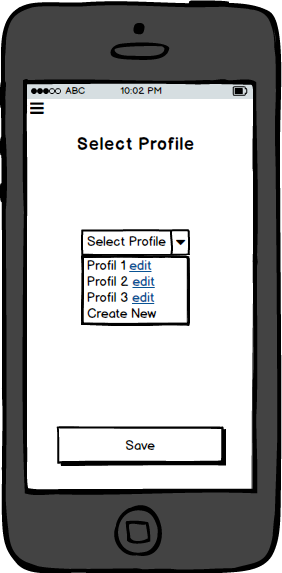
\includegraphics[width=0.20\textwidth]{Profile-1}}
\hfill
\subfigure[Create Profile]{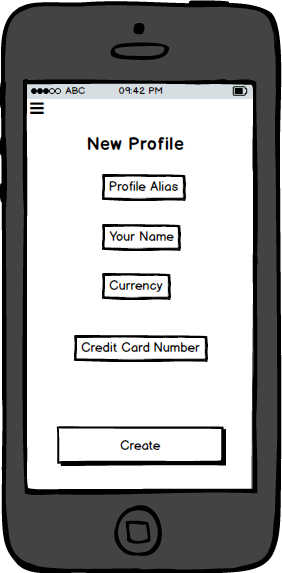
\includegraphics[width=0.20\textwidth]{NewProfile-1}}
\hfill
\subfigure[Edit Profile]{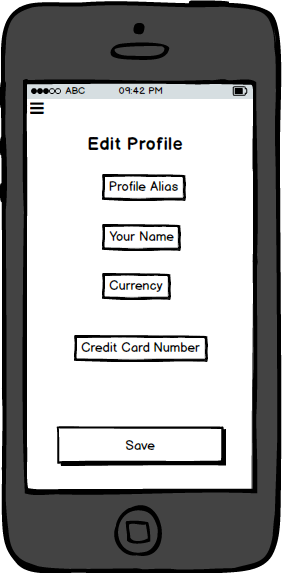
\includegraphics[width=0.20\textwidth]{ChangeProfile-1}}
\vfill
\subfigure[Savetarget erstellen]{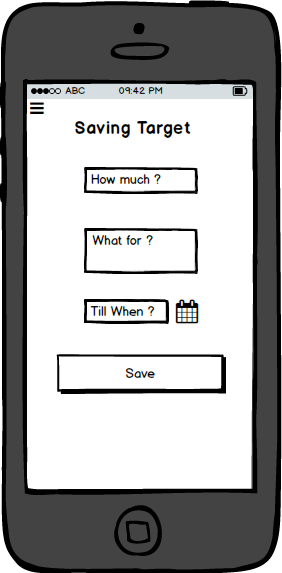
\includegraphics[width=0.20\textwidth]{SavingTarget-1}}
\hfill
\subfigure[Advisor]{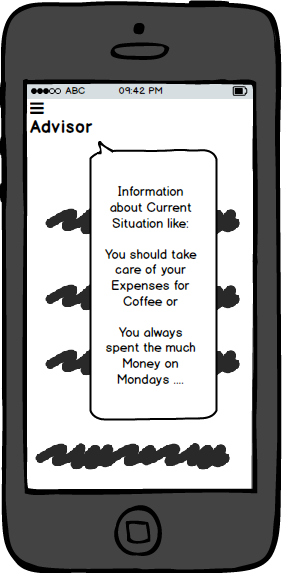
\includegraphics[width=0.20\textwidth]{Advisor-1}}
\end{figure}

\clearpage
\subsection{Prototyp-2}

Der zweite Prototyp unterscheidend sich in Bezug auf den Vorgänger in vielen Punkten. Zur einem haben wir hier den Side Panel abgeschafft und ein Top sowie Bottom Menü eingefügt. Der Vorteil hierbei ist das die punkte stets erreichbar sind und der Nutzer sich das aufklappen des Side Panels ersparen kann. Auch die Fragenstellung, die Anrede selbst, sowie die Eingabe sind freundschaftlicher gestaltet. Hierbei verwenden wir ein Accordion Menü verwendet, welches sich nach Klick auf den jeweiligen Frage aufklappt um entsprechend befüllt zu werden. [j] [k] [l] 

\begin{figure}
\centering
\subfigure[Ausgabe hinzufügen]{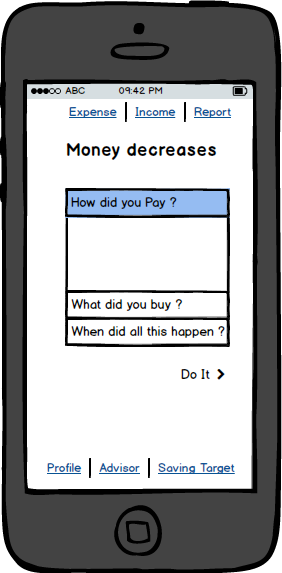
\includegraphics[width=0.15\textwidth]{Expense-2}}
\hfill
\subfigure[Sparziel]{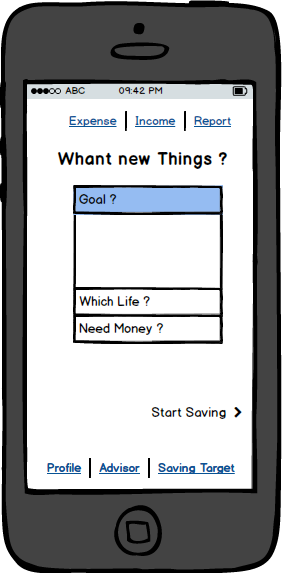
\includegraphics[width=0.15\textwidth]{SavingTarget-2}}
\hfill
\subfigure[Enkommen Speichern]{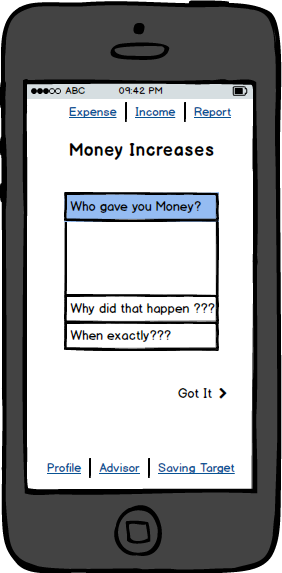
\includegraphics[width=0.15\textwidth]{MoneyIncreases-2}}
\vfill
\subfigure[Select Profil]{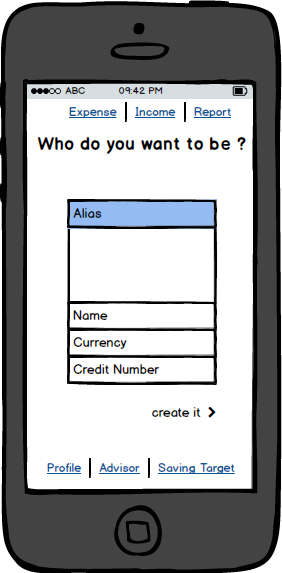
\includegraphics[width=0.15\textwidth]{CreateProfile-2}}
\hfill
\subfigure[Create Profile]{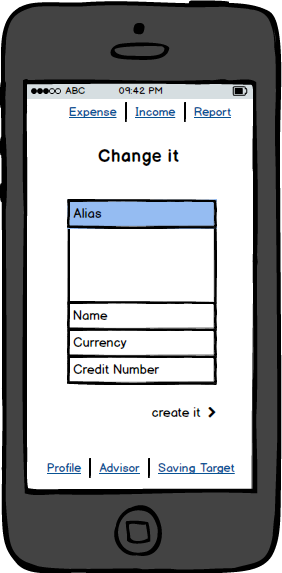
\includegraphics[width=0.15\textwidth]{ChangeProfile-2}}
\hfill
\subfigure[Change Profile]{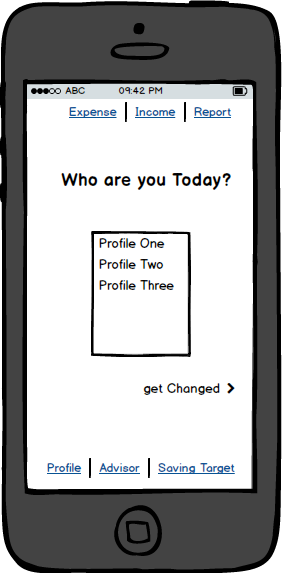
\includegraphics[width=0.15\textwidth]{SelectProfile-2}}
\hfill
\subfigure[Report]{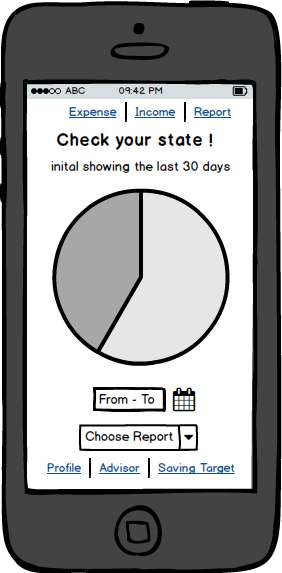
\includegraphics[width=0.15\textwidth]{Report-2}}
\end{figure}

Neben dem freundschaftlichem Touch und auch des Accordion Menüs sind auch die Formulierungen weniger seriös als wie zuvor. Beispiele "Select Profile" [m] oder "Create Profile" [n] bzw. Change Profile [o]. Beim Report haben wir versucht sofort ohne vorherige Abfrage einen initialen Bericht über einen bestimmten Zeitraum zu erstellen. Auch die Datumselektion sollte durch nur einem Feld erleichtert werden. [p]

\clearpage

\subsection{Prototyp-3}

In unserem dritten Prototyp haben wir uns für ein Tab Menü entschieden. Dies sieht zur den beiden Vorgängern zwar etwas überfüllter aus, ist zugleich aber auch strukturierter. [q] Es ermöglicht jedes Feld fast wie eine eigene Seite zu behandeln und würde sehr viel Beschreibung zulassen [r].\\\\ Hierbei haben neben einem horizontalen Tab Menü nämlich auch ein seitlichen Menü eingebaut.[s][t] Der Aktionsbutton (Speichern etc.) befindet sich global im darunter welches die Ansteuerung der Seiten bzw. die Durchführung der Eingaben erleichtern könnte. Dieses Design könnte sich auch bei der Berichterstellung mit einem seitlichen Chart [u] bezahlt machen.\\\\ Die Profile war es bei den Vorgänger notwendig, aufgrund der unterschiedlichen Funktionalitäten (erstellen, selektieren, editieren) eigene Seiten zu erstellen. In diesem Prototyp hat der Nutzer die Möglichkeit, alle relevanten Funktionen, mit nur einem Klick zu erreichen [v]. 

\begin{figure}
\centering
\subfigure[Ausgabe hinzufügen]{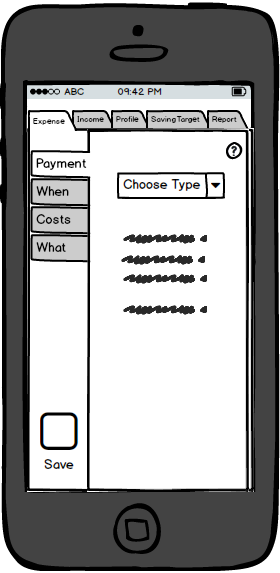
\includegraphics[width=0.15\textwidth]{Expense-3}}
\hfill
\subfigure[Sparziel]{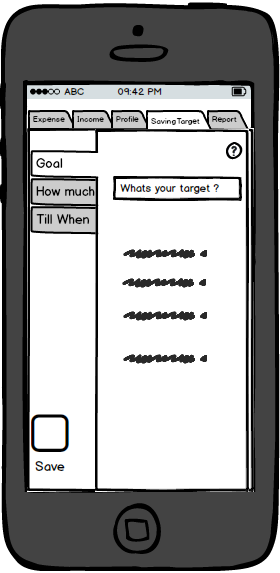
\includegraphics[width=0.15\textwidth]{SaveTarget-3}}
\hfill
\subfigure[Enkommen Speichern]{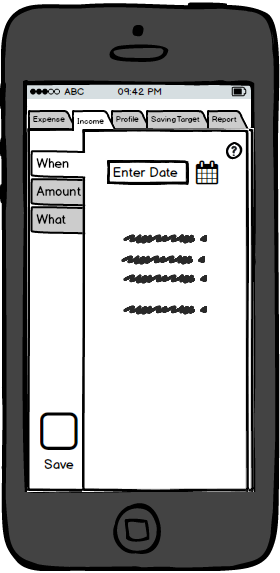
\includegraphics[width=0.15\textwidth]{Income-3}}
\vfill
\subfigure[Change Profile]{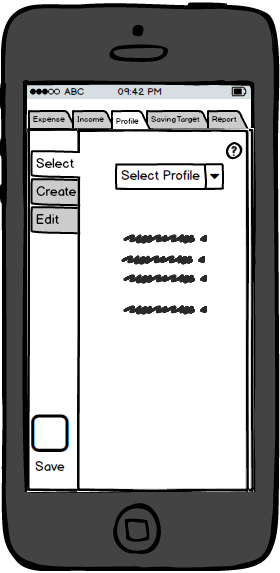
\includegraphics[width=0.15\textwidth]{SelectProfile-3}}
\hfill
\subfigure[Report]{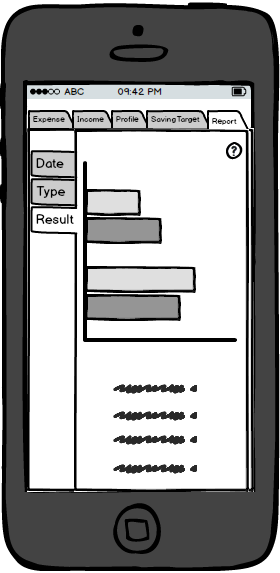
\includegraphics[width=0.15\textwidth]{Report-3}}
\hfill
\subfigure[Select Profil]{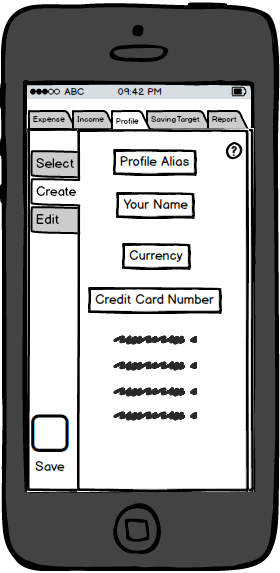
\includegraphics[width=0.15\textwidth]{CreateProfile-3}}
\end{figure}


\clearpage



\section{Interviews}

\subsection{interview - Testuser-1}
\subsection{interview - Testuser-2}
\subsection{interview - Testuser-3}
\clearpage




\begin{thebibliography}{1}
\bibitem{proceeding1} 
\end{thebibliography}


\end{document}